% =====================================================================
% model.tex  (upgraded empirical paper)
% Content: THE model. A recurrent vision transformer with a spatial
% working memory, trained end-to-end with reinforcement learning plus a
% temporal JEPA auxiliary objective (weight 0.5) on a
% cued change-detection task, with element-wise affine memory->vision
% feedback X' = gamma(H) X + beta(H). Presented as a single model
% (no architecture comparison). The task is described conceptually;
% quantitative task/training detail is deferred to Methods.
% =====================================================================

\section{Model}
\label{sec:model}

The model is a recurrent vision transformer with a spatial working
memory, trained end to end from raw pixels with two optimized terms:
reinforcement learning on a cued orientation-change-detection task and a
temporal joint-embedding predictive (JEPA) auxiliary loss (weight $0.5$). It has no
supervised pretraining, no reconstruction objective, and no hand-specified
attention policy. The JEPA head is absent from the forward decision path,
but its gradients shape the shared recurrent representation. The signatures
of primate visual attention reported in Section~\ref{sec:detection} are
learned properties rather than hand-coded attention targets.

This architecture is an RViT+ extension of the empirical Recurrent ViT reported by
Morgan, Albanna, and Herman in 2025 \cite{morgan_albanna_herman2025_rvit}. It is
scientifically distinct from the authors' separate 2026 normative signal-detection
paper on value-directed attention \cite{morgan_albanna_herman2026_vda}; the latter
contains no recurrent transformer, spatial memory, or actor--critic network.

Five components are chained in a single differentiable pipeline
(Figure~\ref{fig:model-schematic}). A convolutional front-end parses each
frame into four patch tokens (Section~\ref{sec:model-frontend}). A
recurrent self-attention encoder lets the tokens interact, with the
recurrent memory feeding back onto the visual tokens through an
element-wise affine modulation (Section~\ref{sec:model-encoder}). A
spatial working memory --- one recurrent cell per location --- integrates
the attended tokens across the trial (Section~\ref{sec:model-memory}). A
distributional actor--critic reads the memory to choose, at every frame,
whether to wait or to declare a change (Section~\ref{sec:model-heads}).
An auxiliary temporal self-distillation head shapes the recurrent
representation without touching the memory or the decision
(Section~\ref{sec:model-jepa}). The whole network is trained by an
off-policy maximum-a-posteriori actor--critic objective with prioritised
episodic replay and an exponential-moving-average target
(Section~\ref{sec:model-training}). We first describe the task at a
conceptual level (Section~\ref{sec:model-task}); the pixel-level
timeline, reward schedule, and training hyperparameters are given in the
Methods (Section~\ref{sec:methods}).

% FIGURE: model schematic. Image sequence -> four 25x25 patches -> conv
% SE-ResNet front-end -> recurrent-ViT self-attention with element-wise
% affine memory->vision feedback -> per-location spatial xLSTM working
% memory -> flattened readout to a distributional QR-DQN actor-critic and
% a JEPA self-distillation head. Render from
% RViT_plus_paper_jepa_conv/repro/figs/fig2_schematic_affine_ew.png.
\begin{figure}[t]
\centering
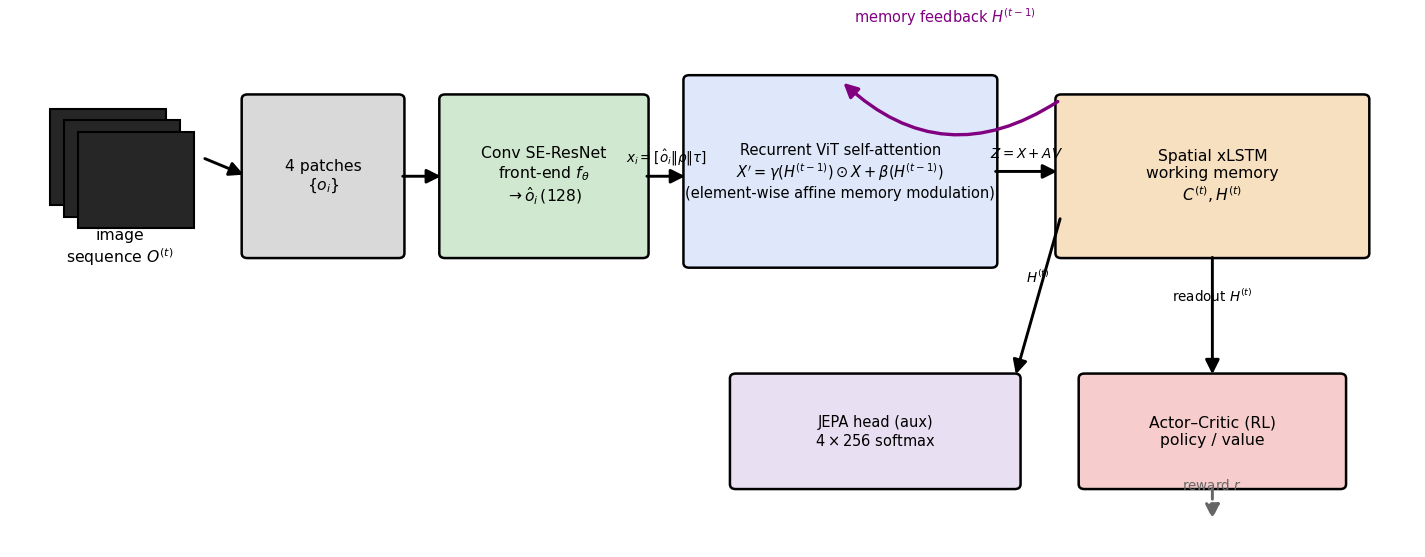
\includegraphics[width=\textwidth]{figures/fig_model_schematic_affine_ew.png}
\caption{\textbf{The model.} A recurrent vision transformer trained by
reinforcement learning on the cued change-detection task plus a temporal JEPA
auxiliary loss (weight $0.5$). Each frame is
split into four patches, encoded by a shared squeeze-and-excitation
convolutional front-end, and passed to a recurrent self-attention
encoder whose visual tokens are affinely modulated by the recurrent
memory before attending to one another. A per-location spatial working
memory integrates the attended tokens across the trial and is read out
to a distributional actor--critic and to an auxiliary self-distillation
head.}
\label{fig:model-schematic}
\end{figure}

% ---------------------------------------------------------------------
\subsection{Task structure}
\label{sec:model-task}

The model performs a covert spatial change-detection task adapted from
the cued-attention paradigms of the primate literature
\cite{posner1980_orienting, MullerFindlay1987,
carrasco2011_visual_attention_25y}. On each trial the model views a short
sequence of images. An initial cue marks one of $\Nloc$ peripheral
locations; a brief delay follows; then $\Nloc$ oriented Gabor patches
appear, one per location, and are held for the remainder of the trial.
On half of trials, at a fixed moment after the patches appear, the
orientation of exactly one patch steps by a magnitude $\Delta$; on the
other half no change occurs. The model must report a change by emitting a
``declare'' action, and is rewarded for declaring after a genuine change
and for withholding through a trial in which no change occurs; declaring
before or without a change ends the trial without reward. Because reward
is earned both for correct detections and for correct rejections, a
conservative always-wait policy is not trivially optimal, and the model
must learn to discriminate a real orientation step from the frame-to-frame
orientation jitter that perturbs every patch.

The cue is not spatially neutral. It carries two pieces of task-relevant
information beyond location, in the spirit of value- and validity-cued
attention \cite{carrasco2011_visual_attention_25y}:
\begin{itemize}
\item \textbf{Value.} The colour of the cue signals the reward that
  detecting a change at the cued location would earn, so that some cued
  changes are worth more than others. This is the substrate for
  \emph{value-directed} attention \cite{failing_theeuwes2018_selection_history,
  hickey2010_reward_salience_acc}.
\item \textbf{Validity.} A ring around the cue signals the probability
  that, given a change, it will occur at the cued location rather than
  elsewhere. This is the substrate for the classic \emph{validity}-graded
  spatial cueing benefit \cite{posner1980_orienting, MullerFindlay1987}.
\end{itemize}
Detecting a change therefore gives the model an opportunity to (i)~orient to the cue,
(ii)~encode the cued location and the cue's value and validity across the
blank while no stimulus is present, and (iii)~monitor the patches for the
one orientation step against a background of noise --- the same demands a
covertly attending primate faces. The single perceptual sensitivity
signal the model can trade across locations is how sharply it resolves a
patch's orientation, so any spatial cueing benefit it exhibits must be
earned through where and how it deploys its internal attention, not
through any built-in preference. The concrete pixel geometry, timing,
cue-colour--to-value map, validity levels, and reward magnitudes are
specified in the Methods (Section~\ref{sec:methods}); here we fix the
number of monitored locations at $\Nloc = 4$ (a $2\times2$ layout), the
setting for the core results, and treat set size as a manipulated
variable in Section~\ref{sec:vda-battery}.

% ---------------------------------------------------------------------
\subsection{Convolutional front-end: pixels to patch tokens}
\label{sec:model-frontend}

Each $50\times50$ RGB frame is split into four $25\times25$ patches, one
per location, in a fixed spatial order so that patch index, cue index,
and change index coincide --- token $i$ always carries location $i$. Each
patch is encoded by a shared squeeze-and-excitation residual
convolutional network (an SE-ResNet stem followed by three residual
stages with a squeeze-and-excitation channel-attention block per stage),
pooled to a $128$-dimensional patch embedding $\hat{o}_i$. The
convolution replaces the pretrained variational encoder of comparable
models with a front-end trained \emph{end to end from pixels} by the
joint reinforcement and temporal-JEPA objective (auxiliary weight $0.5$), with no reconstruction
loss. Two normalisation choices are load-bearing: group
normalisation (rather than batch normalisation) keeps the front-end
stable in the batch-size-one regime of the online recurrent rollout, and
a root-mean-square normalisation (rather than a mean-subtracting layer
normalisation) preserves the uniform colour offset that carries the value
cue, which a mean-subtracting norm would attenuate.

The patch embedding is concatenated with a one-hot spatial-position code
(which location) and a one-hot temporal code (which frame of the trial),
yielding a $140$-dimensional token per patch and a token matrix
$X \in \mathbb{R}^{\Nloc \times 140}$ per frame. The position code makes
each token's location explicit to the self-attention; the temporal code
lets the recurrent memory condition on trial phase --- cue, blank, or
stimulus.

% ---------------------------------------------------------------------
\subsection{Recurrent self-attention with element-wise affine feedback}
\label{sec:model-encoder}

The four patch tokens are contextualised by a single self-attention
layer before entering memory. Crucially, this is a \emph{recurrent}
transformer: the working-memory state $H$ from the previous step feeds
back onto the current visual tokens before they attend to one another.
The feedback is realised as an \emph{element-wise affine modulation} of
the tokens. From the recurrent memory the model computes a low-dimensional
control vector $b = \tanh(\mathrm{bottleneck}(H))$ and, from it, a
per-element scale $\gamma(H)$ and shift $\beta(H)$ of the same shape as
the token matrix, and applies
\begin{equation}
  X' \;=\; \gamma(H) \odot X \;+\; \beta(H),
  \label{eq:affine-feedback}
\end{equation}
where $\odot$ is the element-wise (Hadamard) product. The scale is
initialised to one and the shift to zero, so at the start of training
$X' = X$ and the layer is ordinary self-attention; the memory's ability
to reweight and re-bias each feature of each token is then learned. This
is a diagonal, feature-wise affine transform --- a top-down gain-and-bias
field --- rather than a full matrix mixing of features, which keeps the
feedback interpretable as a per-feature gate. Multiplicative and
additive gain control of this form is the canonical way attention is
thought to act on sensory representations: a feedback signal that scales
the gain of an attended representation and can additively bias it
\cite{reynolds_heeger2009_normalization, mcadams_maunsell1999_v4_tuning,
treue_martinez_trujillo1999_feature_attention}.

The affinely modulated tokens then undergo standard scaled dot-product
self-attention among the $\Nloc$ locations,
\begin{equation}
  Q = X'W_Q,\quad K = X'W_K,\quad V = X'W_V,\qquad
  A = \mathrm{softmax}\!\Big(\tfrac{QK^{\top}}{\sqrt{d}}\Big),\qquad
  Z = X + A\,V,
  \label{eq:self-attention}
\end{equation}
with the raw tokens $X$ retained as a residual so that the current frame
always reaches the memory regardless of the attention weights. The
attention matrix $A \in \mathbb{R}^{\Nloc \times \Nloc}$ --- one weight
per (query location, key location) pair --- is the model's internal,
learned allocation of processing across space, and it is the quantity we
read out and manipulate throughout the results: its row-marginal
$\alpha_i$, the share of attention placed on location $i$, is the
model-internal analogue of the attentional weight in the psychophysical
and physiological literature \cite{carrasco2011_visual_attention_25y,
reynolds_heeger2009_normalization}. Because the memory drives the
modulation~(\ref{eq:affine-feedback}) that in turn shapes $Q$, $K$, and
$V$, the allocation $A$ is jointly determined by the incoming image and
the maintained top-down state --- exactly the recurrent, feedback-driven
account of attention that motivates the architecture
\cite{ghose_maunsell2002_task_timing, sani2017_temporal_v4_gain}. We
supply a differentiable clamp on the pre-softmax attention logits that
lets us, in analysis, drive attention toward or away from a chosen
location; this is the lever behind the causal ``stimulation'' experiments
of Section~\ref{sec:detection} and is inert during training.

% ---------------------------------------------------------------------
\subsection{Spatial working memory}
\label{sec:model-memory}

The contextualised tokens $Z$ are integrated across the trial by a
spatial working memory: an extended LSTM (xLSTM) cell applied
\emph{per location}, with a shared parameterisation but a private state
per patch, producing a $128$-dimensional memory vector $H_i$ for each of
the $\Nloc$ locations. The xLSTM's stabilised, exponential input and
forget gates give it a controllable retention time-constant, so it can
integrate cue information across the stimulus-free blank and accumulate weak
orientation evidence across the stimulus frames
--- the two demands the task imposes on memory. Maintaining one recurrent
state per location keeps the memory spatially addressable: the model can,
and does, store what it has seen at each monitored location separately,
which is what makes location-specific processing and change localisation
possible. The memory state at frame $t$ is the $H$
that drives the affine feedback~(\ref{eq:affine-feedback}) at frame
$t+1$, closing the perception--memory loop.

% ---------------------------------------------------------------------
\subsection{Decision: distributional actor--critic}
\label{sec:model-heads}

The per-location memory vectors are flattened into a single
$\Nloc \times 128 = 512$-dimensional readout --- the model discards the
spatial structure at the decision stage --- and passed to two heads that
share no parameters. The \emph{actor} maps the readout through a
feed-forward trunk to logits over two actions, \emph{wait} and
\emph{declare-change}, and is biased at initialisation toward waiting so
that the model does not begin by declaring on every frame. The
\emph{critic} is distributional: rather than a single scalar value it
predicts a small set of return quantiles per action (a quantile-regression
value head), from which the state value is recovered as the
action-probability-weighted mean. At every frame the model thus emits a
full action distribution and a distributional value, and the trajectory
of these quantities across a trial --- in particular the jump in
predicted value at the moment of the change --- is one of the readouts we
analyse in Section~\ref{sec:detection}. The decision is made online, frame
by frame: the model chooses whether to declare as soon as it has
integrated enough evidence, which is what gives it a reaction time and
hence a chronometric function to compare against behaviour.

% ---------------------------------------------------------------------
\subsection{Auxiliary temporal self-distillation}
\label{sec:model-jepa}

A joint-embedding predictive self-distillation head (a temporal V-JEPA
objective with DINO-style centering) shapes the recurrent representation.
It reads the memory cell at each location and predicts, for the same
location one frame ahead, the soft assignment produced by an
exponential-moving-average teacher copy of the network, over a set of
learned prototypes. The head has no direct forward connection to the actor, critic, attention
logits, or next recurrent state. It nevertheless participates in the total
optimized loss with weight $0.5$, so its gradients shape the representation
that those components use. The measured attentional signatures therefore
arise under joint reinforcement and temporal self-supervision; the present
experiments do not apportion their training-time contribution between the
two losses.

% ---------------------------------------------------------------------
\subsection{Training}
\label{sec:model-training}

The network is trained with an off-policy actor--critic objective from sparse
task reward plus the temporal JEPA auxiliary objective (weight $0.5$). The actor is updated by a
maximum-a-posteriori policy-optimisation step (an expectation step that
reweights actions by their advantage under an exponential-moving-average
reference policy, together with a behavioural-cloning term), and the
distributional critic by a quantile-regression temporal-difference loss.
Learning is stabilised by three standard ingredients: prioritised
\emph{episodic} replay, so that informative whole trials are revisited in
proportion to their surprise; an exponential-moving-average target
network that supplies both the critic bootstrap target and the actor's
reference policy; and a curriculum on task difficulty that shrinks the
orientation-change magnitude only after the model reliably solves the
current level, so the model is always trained near the edge of its
competence. All hyperparameters, the exact objective, and the curriculum
schedule are given in the Methods (Section~\ref{sec:methods}). The core causal analyses use one canonical affine-feedback $d_{\mathrm{mem}}=128$
checkpoint. The set-size and task-variant sections instead compare separately trained
checkpoints that share the affine-feedback mechanism but not their learned weights;
Methods records the relevant geometry and training-support differences.

% ---------------------------------------------------------------------
\subsection{What the trained model does, in brief}
\label{sec:model-summary}

Trained to competence, the model is correct on $\approx 0.83$ of trials,
producing orderly sigmoidal psychometric functions and monotone
chronometric functions --- response rate rises with the change magnitude
$\Delta$, floors near the false-alarm rate at $\Delta = 0$, and approaches
the upper end of the sampled response range by roughly $30^\circ$, while reaction time falls as $\Delta$
grows.\footnote{Behavioural summary statistics are quoted from the model
analyses of Section~\ref{sec:detection}; the operating point corresponds to
a curriculum-hardened difficulty level.} Its internal attention follows
an interpretable schedule across the trial: it orients to the cue (placing
$\approx 0.73$ of its attention on the cued location at the cue frame in the
canonical VDA4 checkpoint,
against a uniform baseline of $0.25$), releases toward baseline during the
blank ($\approx 0.22$), re-acquires the cued location as the patches
appear ($0.44 \!\to\! 0.80$ over the stimulus frames), and locks onto a
patch whose orientation steps ($\to 1.00$ for a cued change on the change
frame). Cue value is decoded from the memory at the cue frame and remains recoverable
for the rest of the trial, while change presence and location become sharply
decodable at the change frame. No cue-location decoder was fitted across the
delay; the later cue-directed re-acquisition of attention is therefore indirect
evidence compatible with, but not proof of, spatial maintenance. These are the
raw signatures we develop, quantify,
and probe causally in Section~\ref{sec:detection}: a genuine spatial cueing
benefit, an attention-dependent shift of the signal-detection criterion
and sensitivity, and a value-graded decision learned under the joint objective.
